\chapter*{引言}

无论即将到来的是大数据时代还是人工智能时代,亦或是传统行业使用人工智能在云上处理大数据的时代,作为一个有理想有追求的程序员,不懂深度学习(Deep Learning)这个超热的技术,会不会感觉马上就out了?现在救命稻草来了,《零基础入门深度学习》系列文章旨在讲帮助爱编程的你从零基础达到入门级水平。零基础意味着你不需要太多的数学知识,只要会写程序就行了,没错,这是专门为程序员写的文章。虽然文中会有很多公式你也许看不懂,但同时也会有更多的代码,程序员的你一定能看懂的(我周围是一群狂热的Clean Code程序员,所以我写的代码也不会很差)。

这个笔记主要是 Bingtao Han\footnote{\textbf{版权:}本文的版权归Bingtao Han所有。} \href{https://www.zybuluo.com/hanbingtao/note/433855}{《零基础入门深度学习》}的 \LaTeX{} 版本,文中的所有代码都发布\href{https://github.com/hanbt/learn_dl}{\textbf{Github}}上。




\chapter{感知器}\label{chap:Per}

\begin{introduction}
	\item 深度学习是啥~\ref{Per:1}
	\item 感知器~\ref{Per:2}
	\item 感知器的定义~\ref{Per:3}
	\item 感知器还能做什么~\ref{Per:4}
	\item 编程实战:实现感知器~\ref{Per:5}
\end{introduction}

\section{深度学习是啥}\label{Per:1}

在人工智能领域,有一个方法叫机器学习。在机器学习这个方法里,有一类算法叫神经网络。神经网络如下图所示:

\begin{figure}[htbp]
	\centering
	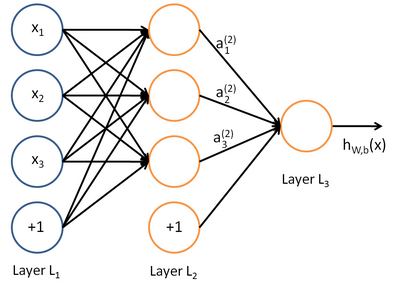
\includegraphics[width=0.5\textwidth]{Perceptron1.png}
	\caption{神经网络}
	\label{fig:Per0}
\end{figure}

图\ref{fig:Per0}中每个圆圈都是一个神经元,每条线表示神经元之间的连接。我们可以看到,上面的神经元被分成了多层,层与层之间的神经元有连接,而层内之间的神经元没有连接。最左边的层叫做\textbf{输入层},这层负责接收输入数据;最右边的层叫\textbf{输出层},我们可以从这层获取神经网络输出数据。输入层和输出层之间的层叫做\textbf{隐藏层}。

隐藏层比较多(大于2)的神经网络叫做深度神经网络。而深度学习,就是使用深层架构(比如,深度神经网络)的机器学习方法。

那么深层网络和浅层网络相比有什么优势呢?简单来说深层网络能够表达力更强。事实上,一个仅有一个隐藏层的神经网络就能拟合任何一个函数,但是它需要很多很多的神经元。而深层网络用少得多的神经元就能拟合同样的函数。也就是为了拟合一个函数,要么使用一个浅而宽的网络,要么使用一个深而窄的网络。而后者往往更节约资源。

深层网络也有劣势,就是它不太容易训练。简单的说,你需要大量的数据,很多的技巧才能训练好一个深层网络。这是个手艺活。


\section{感知器}\label{Per:2}
看到这里,如果你还是一头雾水,那也是很正常的。为了理解神经网络,我们应该先理解神经网络的组成单元------\textbf{神经元}。神经元也叫做\textbf{感知器}。感知器算法在上个世纪50-70年代很流行,也成功解决了很多问题。并且,感知器算法也是非常简单的。

\subsection{感知器的定义}\label{Per:3}

下图是一个感知器:

\begin{figure}[htbp]
	\centering
	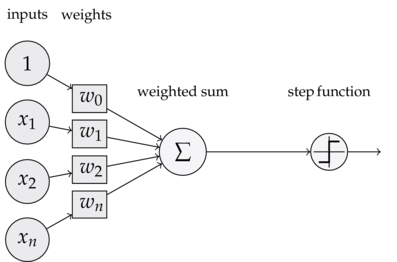
\includegraphics[width=0.5\textwidth]{Perceptron2.png}
	\caption{感知器}
\end{figure}

可以看到,一个感知器有如下组成部分:

\begin{itemize}
	\item
	      \textbf{输入权值}
	      一个感知器可以接收多个输入$(x_1, x_2,...,x_n\mid x_i\in\Re)$,每个输入上有一个\textbf{权值}$w_i\in\Re$,此外还有一个\textbf{偏置项}$b\in\Re$,就是上图中$w_0$。
	\item
	      \textbf{激活函数}
	      感知器的激活函数可以有很多选择,比如我们可以选择下面这个\textbf{阶跃函数}$f$来作为激活函数:
	      \begin{equation*}
		      f(x)=\left\{
		      \begin{aligned}
			      1 & \quad z>0       \\
			      0 & \quad otherwise
		      \end{aligned}
		      \right.
	      \end{equation*}
	\item
	      \textbf{输出} 感知器的输出由下面这个公式来计算
	      \begin{equation}
		      \label{eq:Per1}
		      y=f(w \bullet x + b)
	      \end{equation}
\end{itemize}

如果看完上面的公式一下子就晕了,不要紧,我们用一个简单的例子来帮助理解。

\begin{example}
	用感知器实现 \textcolor{main}{\textbf{and}} 函数
\end{example}

我们设计一个感知器,让它来实现 \textcolor{main}{\textbf{and}} 运算。程序员都知道,\textcolor{main}{\textbf{and}} 是一个二元函数(带有两个参数$x_1$和$x_2$),下面是它的\textbf{真值表}:


\begin{table}[htbp]
	\centering
	\setlength{\tabcolsep}{10mm}
	\caption{\textcolor{main}{\textbf{and}}真值表}
	\begin{tabular}{ccc}
		\hline
		$x_1$ & $x_2$ & $y$ \\ \hline
		0     & 0     & 0   \\
		0     & 1     & 0   \\
		1     & 0     & 0   \\
		1     & 1     & 1   \\ \hline
	\end{tabular}
	\label{tab:Per1}
\end{table}

为了计算方便,我们用0表示\textbf{false},用1表示\textbf{true}。这没什么难理解的,对于C语言程序员来说,这是天经地义的。

我们令$w_1=0.5;w_2=0.5;b=-0.8$,而激活函数$f$就是前面写出来的\textbf{阶跃函数},这时,感知器就相当于\textcolor{main}{\textbf{and}} 函数。不明白?我们验算一下:

输入上面真值表的第一行,即$x_1=0;x_2=0$,那么根据公式\ref{eq:Per1},计算输出:
\begin{align*}
	y & =f(w \bullet x + b) = f(w_1x_1+w_2x_2+b)    \\
	  & =f(0.5\times0+0.5\times0-0.8) = f(-0.8) = 0
\end{align*}
也就是当$x_1, x_2$都为0的时候,$y$为0,这就是表\ref{tab:Per1}的第一行。读者可以自行验证上述真值表的第二、三、四行。

\begin{example}
	用感知器实现 \textcolor{main}{\textbf{or}} 函数
\end{example}

同样,我们也可以用感知器来实现\textcolor{main}{\textbf{or}}运算。仅仅需要把偏置项$b$的值设置为$-0.3$就可以了。我们验算一下,下面是\textcolor{main}{\textbf{or}}运算的\textbf{真值表}:


\begin{table}[htbp]
	\centering
	\setlength{\tabcolsep}{10mm}
	\caption{\textcolor{main}{\textbf{or}}真值表}
	\begin{tabular}{ccc}
		\hline
		$x_1$ & $x_2$ & $y$ \\ \hline
		0     & 0     & 0   \\
		0     & 1     & 1   \\
		1     & 0     & 1   \\
		1     & 1     & 1   \\ \hline
	\end{tabular}
	\label{tab:Per2}
\end{table}


我们来验算第二行,这时的输入是$x_1=0;x_2=1$,带入公式\ref{eq:Per1}:
\begin{align*}
	y & =f(w \bullet x + b) = f(w_1x_1+w_2x_2+b)   \\
	  & =f(0.5\times1+0.5\times0-0.3) = f(0.2) = 1
\end{align*}
也就是当$x_1=0;x_2=1$时,$y$为1,即表\ref{tab:Per2}第二行。读者可以自行验证其它行。


\subsection{感知器还能做什么}\label{Per:4}

事实上,感知器不仅仅能实现简单的布尔运算。它可以拟合任何的线性函数,任何\textbf{线性分类}或\textbf{线性回归}问题都可以用感知器来解决。前面的布尔运算可以看作是\textbf{二分类}问题,即给定一个输入,输出0(属于分类0)或1(属于分类1)。如图\ref{fig:Per1_a}所示,\textcolor{main}{\textbf{and}}运算是一个线性分类问题,即可以用一条直线把分类0(false,红叉表示)和分类1(true,绿点表示)分开。
然而,感知器却不能实现异或运算,如图\ref{fig:Per1_b}所示,异或运算不是线性的,你无法用一条直线把分类0和分类1分开。

\begin{figure}[htbp]
	\centering
	\subfigure[]{
		\begin{minipage}[t]{0.5\linewidth}
			\centering
			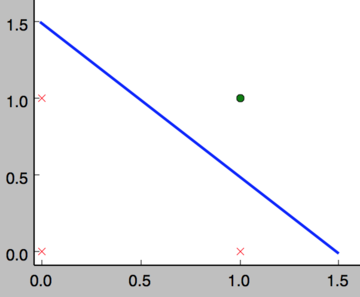
\includegraphics[width=2in]{Perceptron3.png}
			\label{fig:Per1_a}
			%\caption{fig1}
		\end{minipage}%
	}%
	\subfigure[]{
		\begin{minipage}[t]{0.5\linewidth}
			\centering
			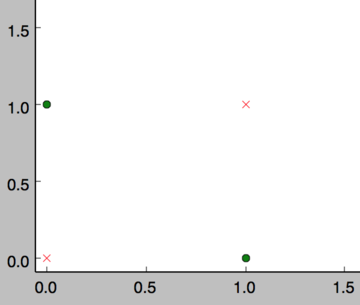
\includegraphics[width=2in]{Perceptron4.png}
			\label{fig:Per1_b}
			%\caption{fig2}
		\end{minipage}%
	}%
	\centering
	\caption{真值图}
	\label{fig:Per1}
\end{figure}


\subsection{感知器的训练}\label{Per:4}

现在,你可能困惑前面的权重项和偏置项的值是如何获得的呢?这就要用到感知器训练算法:将权重项和偏置项初始化为0,然后,利用下面的\textbf{感知器规则}迭代的修改$w_i$和$b$,直到训练完成。
\begin{align*}
	w_i & \gets w_i+\Delta w_i \\
	b   & \gets b+\Delta b
\end{align*}
其中:
\begin{align*}
	\Delta w_i & =\eta(t-y)x_i \\
	\Delta b   & =\eta(t-y)
\end{align*}

$w_i$是与输入$x_i$对应的权重项,$b$是偏置项。事实上,可以把$b$看作是值永远为1的输入$x_b$所对应的权重。$t$是训练样本的\textbf{实际值},一般称之为\textbf{label}。而$y$是感知器的输出值,它是根据公式\ref{eq:Per1}计算得出。$\eta$是一个称为\textbf{学习速率}的常数,其作用是控制每一步调整权的幅度。

每次从训练数据中取出一个样本的输入向量$x$,使用感知器计算其输出$y$,再根据上面的规则来调整权重。每处理一个样本就调整一次权重。经过多轮迭代后(即全部的训练数据被反复处理多轮),就可以训练出感知器的权重,使之实现目标函数。


\section{编程实战:实现感知器}\label{Per:5}

\begin{note}
	完整代码请参考GitHub: \url{https://github.com/hanbt/learn_dl/blob/master/perceptron.py}
	(python2.7)
\end{note}


对于程序员来说,没有什么比亲自动手实现学得更快了,而且,很多时候一行代码抵得上千言万语。接下来我们就将实现一个感知器。

下面是一些说明:
\begin{itemize}
	\item
	      使用python语言。python在机器学习领域用的很广泛,而且,写python程序真的很轻松。
	\item
	      面向对象编程。面向对象是特别好的管理复杂度的工具,应对复杂问题时,用面向对象设计方法很容易将复杂问题拆解为多个简单问题,从而解救我们的大脑。
	\item
	      没有使用numpy。numpy实现了很多基础算法,对于实现机器学习算法来说是个必备的工具。但为了降低读者理解的难度,下面的代码只用到了基本的python(省去您去学习numpy的时间)。
\end{itemize}


下面是感知器类的实现,非常简单。去掉注释只有27行,而且还包括为了美观(每行不超过60个字符)而增加的很多换行。
\begin{lstlisting}
class Perceptron(object):
    def __init__(self, input_num, activator):
        '''
        初始化感知器,设置输入参数的个数,以及激活函数。
        激活函数的类型为double -> double
        '''
        self.activator = activator
        # 权重向量初始化为0
        self.weights = [0.0 for _ in range(input_num)]
        # 偏置项初始化为0
        self.bias = 0.0
    def __str__(self):
        '''
        打印学习到的权重、偏置项
        '''
        return 'weights\t:%s\nbias\t:%f\n' % (self.weights, self.bias)
    def predict(self, input_vec):
        '''
        输入向量,输出感知器的计算结果
        '''
        # 把input_vec[x1,x2,x3...]和weights[w1,w2,w3,...]打包在一起
        # 变成[(x1,w1),(x2,w2),(x3,w3),...]
        # 然后利用map函数计算[x1*w1, x2*w2, x3*w3]
        # 最后利用reduce求和
        return self.activator(
            reduce(lambda a, b: a + b,
                   map(lambda (x, w): x * w,  
                       zip(input_vec, self.weights))
                , 0.0) + self.bias)
    def train(self, input_vecs, labels, iteration, rate):
        '''
        输入训练数据:一组向量、与每个向量对应的label;以及训练轮数、学习率
        '''
        for i in range(iteration):
            self._one_iteration(input_vecs, labels, rate)
    def _one_iteration(self, input_vecs, labels, rate):
        '''
        一次迭代,把所有的训练数据过一遍
        '''
        # 把输入和输出打包在一起,成为样本的列表[(input_vec, label), ...]
        # 而每个训练样本是(input_vec, label)
        samples = zip(input_vecs, labels)
        # 对每个样本,按照感知器规则更新权重
        for (input_vec, label) in samples:
            # 计算感知器在当前权重下的输出
            output = self.predict(input_vec)
            # 更新权重
            self._update_weights(input_vec, output, label, rate)
    def _update_weights(self, input_vec, output, label, rate):
        '''
        按照感知器规则更新权重
        '''
        # 把input_vec[x1,x2,x3,...]和weights[w1,w2,w3,...]打包在一起
        # 变成[(x1,w1),(x2,w2),(x3,w3),...]
        # 然后利用感知器规则更新权重
        delta = label - output
        self.weights = map(
            lambda (x, w): w + rate * delta * x,
            zip(input_vec, self.weights))
        # 更新bias
        self.bias += rate * delta
\end{lstlisting}


接下来,我们利用这个感知器类去实现\textcolor{main}{\textbf{and}}函数。
\begin{lstlisting}
def f(x):
    '''
    定义激活函数f
    '''
    return 1 if x > 0 else 0
def get_training_dataset():
    '''
    基于and真值表构建训练数据
    '''
    # 构建训练数据
    # 输入向量列表
    input_vecs = [[1,1], [0,0], [1,0], [0,1]]
    # 期望的输出列表,注意要与输入一一对应
    # [1,1] -> 1, [0,0] -> 0, [1,0] -> 0, [0,1] -> 0
    labels = [1, 0, 0, 0]
    return input_vecs, labels    
def train_and_perceptron():
    '''
    使用and真值表训练感知器
    '''
    # 创建感知器,输入参数个数为2(因为and是二元函数),激活函数为f
    p = Perceptron(2, f)
    # 训练,迭代10轮, 学习速率为0.1
    input_vecs, labels = get_training_dataset()
    p.train(input_vecs, labels, 10, 0.1)
    #返回训练好的感知器
    return p
if __name__ == '__main__': 
    # 训练and感知器
    and_perception = train_and_perceptron()
    # 打印训练获得的权重
    print and_perception
    # 测试
    print '1 and 1 = %d' % and_perception.predict([1, 1])
    print '0 and 0 = %d' % and_perception.predict([0, 0])
    print '1 and 0 = %d' % and_perception.predict([1, 0])
    print '0 and 1 = %d' % and_perception.predict([0, 1])
\end{lstlisting}

将上述程序保存为perceptron.py文件,通过命令行执行这个程序,其运行结果为:

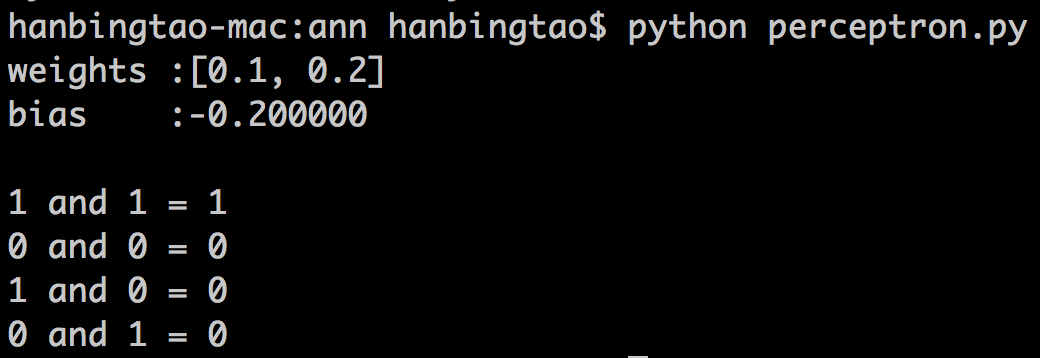
\includegraphics[width=0.8\textwidth]{Perceptron5.png}

神奇吧!感知器竟然完全实现了\textcolor{main}{\textbf{and}}函数。读者可以尝试一下利用感知器实现其它函数。

\section{小结}

终于看(写)到小结了...,大家都累了。对于零基础的你来说,走到这里应该已经很烧脑了吧。没关系,休息一下。值得高兴的是,你终于已经走出了深度学习入门的第一步,这是巨大的进步;坏消息是,这仅仅是最简单的部分,后面还有无数艰难险阻等着你。不过,你学的困难往往意味着别人学的也困难,掌握一门高门槛的技艺,进可糊口退可装逼,是很值得的。

下一篇文章,我们将讨论另外一种感知器:\textbf{线性单元},并由此引出一种可能是最最重要的优化算法:\textbf{梯度下降}算法。